
\documentclass[hidelinks, a4paper, 12pt]{report}
\usepackage{tocbibind}
\usepackage{fancyhdr}
\setlength{\headheight}{15pt}
\pagestyle{fancy}
\fancyhf{}
\fancyhead[L]{\leftmark}
\fancyhead[R]{\thepage}
\usepackage[top=1.5cm, bottom=2cm]{geometry}
\setlength{\tolerance}{1}
\setlength{\emergencystretch}{\maxdimen}
\setlength{\hyphenpenalty}{10000}
\setlength{\hbadness}{10000}

\usepackage[unicode]{hyperref}
\usepackage[LGR, T1]{fontenc}
\usepackage[utf8]{inputenc}
\usepackage[english, greek]{babel}
\usepackage{alphabeta}
\usepackage{csquotes}
\usepackage{dirtytalk}

\usepackage[backend=biber, style=numeric, natbib=true, sorting=none]{biblatex}
\addbibresource{bibliography.bib}

\usepackage{graphicx}
\usepackage{caption}
\usepackage{subcaption}

\usepackage{indentfirst}
\setlength{\parindent}{2em}
\setlength{\parskip}{1em}

\title{Διαδραστικό \foreignlanguage{english}{Pipeline} Ανάλυσης σε δεδομένα Μοριακής Βιολογίας}
\author{Χρήστος Σπυρίδων Καρύδης - \foreignlanguage{english}{inf2022076}\\ Ευαγγελία Φώτη - \foreignlanguage{english}{inf2022224}\\ Ευτυχία Φίλιου - Π2019202}

\begin{document}

\newgeometry{top=1.5cm, bottom=2.0cm}

\begin{titlepage}
    \newcommand{\HRule}{\rule{\linewidth}{0.5mm}}
    \center 
    
\includegraphics[width=0.6\linewidth]{title/ionian_university_logo.png}\\[0.5cm]
    \textsl{\Huge Ιόνιο Πανεπιστήμιο}\\[0.5cm] 
    \textsl{\Large Τμήμα Πληροφορικής}\\[2cm] 
    \makeatletter
    \HRule \\[0.6cm]
    {\huge \bfseries \@title}\\[0.3cm]
    \HRule \\[2cm]
    \large
    
    \begin{minipage}{0.45\textwidth}
    	\begin{flushleft}
            \emph{Συγγραφείς:}\\
            \@author \\
        \end{flushleft}
    \end{minipage}
    ~
    \begin{minipage}{0.45\textwidth}
    	\begin{flushright}
            \emph{Υπεύθυνος Καθηγητής:} \\
            \textup{Αριστείδης Βραχάτης}
        \end{flushright}
    \end{minipage}\\[3cm]
    
    \makeatother
    
    {\large Η εργασία κατατέθηκε για το μάθημα:}\\[0.2cm]
    {\Large \emph{Τεχνολογίες Λογισμικού 2025}}\\[1cm]
    {\large Μάιος 2025}\\[2cm]
    \vfill 
\end{titlepage}

\restoregeometry


\selectlanguage{greek}
\renewcommand{\contentsname}{Περιεχόμενα}
\renewcommand{\listfigurename}{Λίστα Σχημάτων}
\renewcommand{\listtablename}{Λίστα Πινάκων}
\renewcommand{\chaptername}{Κεφάλαιο}
\renewcommand{\appendixname}{Παράρτημα}
\renewcommand{\bibname}{Βιβλιογραφία}

\pagenumbering{roman}
\setlength{\parskip}{0.5em}
\tableofcontents
\newpage

\pagenumbering{arabic}
\setlength{\parskip}{1em}

\chapter*{Περίληψη}

Η παρούσα εργασία παρουσιάζει μια διαδραστική εφαρμογή ανάλυσης δεδομένων μοριακής βιολογίας \foreignlanguage{english}{(scRNA-seq)}, υλοποιημένη σε περιβάλλον \foreignlanguage{english}{Streamlit}. Η εφαρμογή επιτρέπει την παραμετροποιημένη ανάλυση με ενσωματωμένες τεχνικές προεπεξεργασίας, \foreignlanguage{english}{PCA, UMAP, clustering}, διόρθωση \foreignlanguage{english}{batch effect} με \foreignlanguage{english}{Harmony}, καθώς και ανάλυση διαφορικής γονιδιακής έκφρασης. Οι χρήστες μπορούν εύκολα να ανεβάζουν αρχεία τύπου \foreignlanguage{english}{`.h5ad`}, να ρυθμίζουν τις παραμέτρους, να εκτελούν ανάλυση και να εξάγουν αποτελέσματα και οπτικοποιήσεις. Η εφαρμογή συνοδεύεται από δυνατότητα \foreignlanguage{english}{dockerization} για εύκολη μεταφορά και αναπαραγωγή σε κάθε σύστημα και από τα \foreignlanguage{english}{UML} διαγράμματα \foreignlanguage{english}{(Class Diagram \& Use Case Diagram)} που περιγράφουν την αρχιτεκτονική και τη λειτουργικότητα της εφαρμογής.
\chapter{Εισαγωγή}

Η ανάλυση δεδομένων μονοκυτταρικής ακολουθίας \foreignlanguage{english}{RNA} \foreignlanguage{english}{(single-cell RNA sequencing / scRNA-seq)} αποτελεί σημαντική πρόοδο στη βιοπληροφορική, επιτρέποντας τη μελέτη της έκφρασης γονιδίων σε μεμονωμένα κύτταρα. Η ποικιλομορφία των κυτταρικών τύπων και η ανάγκη ανακάλυψης νέων κυτταρικών υποπληθυσμών απαιτεί την ύπαρξη διαδραστικών εργαλείων, τα οποία επιτρέπουν οπτικοποίηση και επεξεργασία των δεδομένων με εύχρηστο τρόπο. Στο πλαίσιο του μαθήματος Τεχνολογίες Λογισμικού (2025), αναπτύχθηκε μια εφαρμογή βασισμένη σε \foreignlanguage{english}{Streamlit}, η οποία συνδυάζει τα στάδια ανάλυσης \foreignlanguage{english}{scRNA-seq} σε ενιαίο γραφικό περιβάλλον.
\chapter{Σχεδιασμός της Υλοποίησης}

Η εφαρμογή οργανώνεται σε έξι βασικά \foreignlanguage{english}{tabs}, τα οποία αντιστοιχούν στα στάδια της ανάλυσης:

\begin{itemize}
  \item \textbf{Δεδομένα:} Ανέβασμα αρχείων τύπου \foreignlanguage{english}{`.h5ad`} και προεπισκόπηση μεταδεδομένων και γονιδίων.
  \item \textbf{Προεπεξεργασία:} Φιλτράρισμα κυττάρων/γονιδίων, αφαίρερση \foreignlanguage{english}{MT-, ERCC} γονιδίων, κανονικοποίηση, \foreignlanguage{english}{log1p, HVG} επιλογή και \foreignlanguage{english}{scaling}.
  \item \textbf{Ανάλυση:} \foreignlanguage{english}{PCA, clustering} με \foreignlanguage{english}{Leiden, UMAP (2D/3D)}, και επιλογή χρήσης ή μη \foreignlanguage{english}{Harmony}.
  \item \textbf{Γονιδιακή Ανάλυση:} Ανάληση \foreignlanguage{english}{marker genes} και \foreignlanguage{english}{DEG (Differential Expression)} με διάφορες οπτικοποιήσεις.
  \item \textbf{Εξαγωγή:} Κατεβάσματα \foreignlanguage{english}{preprocessed} αρχείων, \foreignlanguage{english}{DEGs} σε \foreignlanguage{english}{CSV/XLSX}, \foreignlanguage{english}{Volcano plots, Heatmap, Dotplot, Violin} και \foreignlanguage{english}{UMAP} εικόνες.
  \item \textbf{Ομάδα:} Παρουσίαση μελών ομάδας και των ρόλων τους.
\end{itemize}

Η εφαρμογή βασίζεται στο \foreignlanguage{english}{Streamlit} και αξιοποιεί \foreignlanguage{english}{`session state`} για μεταφορά δεδομένων μεταξύ των \foreignlanguage{english}{tabs}, ενώ κάθε βήμα ελέγχεται με παραμετρικά \foreignlanguage{english}{sliders} και επιλογές που ενημερώνουν δυναμικά την επόμενη ενέργεια.
\chapter{\foreignlanguage{english}{UML} Διαγράμματα}

Στην παρούσα ενότητα παρουσιάζονται δύο βασικά διαγράμματα \foreignlanguage{english}{UML} για την τεκμηρίωση της λειτουργικότητας και της αρχιτεκτονικής της εφαρμογής.

Το \foreignlanguage{english}{\textbf{Class Diagram}} απεικονίζει τις κύριες κλάσεις και τις μεταξύ τους σχέσεις, με έμφαση στη ροή δεδομένων και τις κύριες μεθόδους.

\begin{figure}[h]
    \centering
    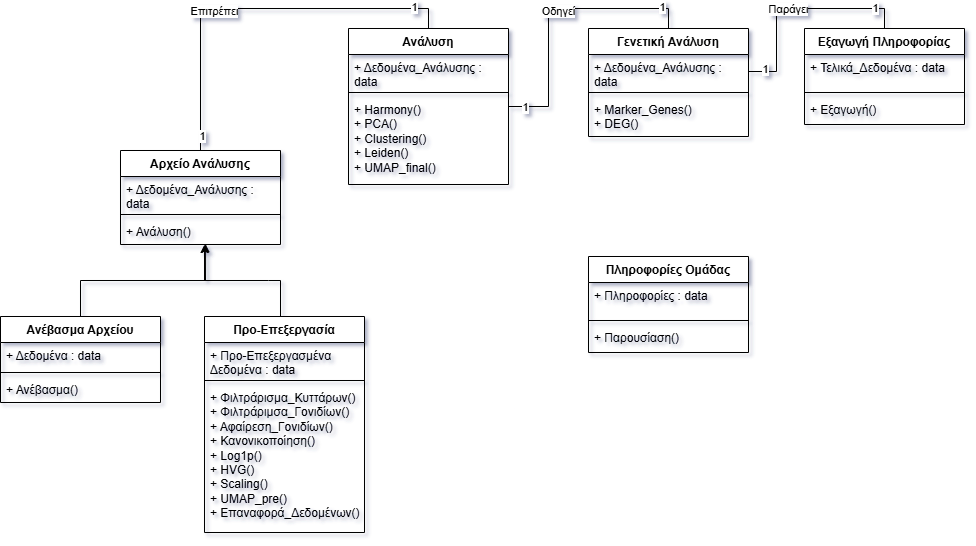
\includegraphics[width=0.95\textwidth]{images/Class_Diagram.png}
    \caption{\foreignlanguage{english}{UML Class Diagram} της εφαρμογής}
\end{figure}

\newpage

Το \foreignlanguage{english}{\textbf{Use Case Diagram}} περιγράφει τις ενέργειες που εκτελεί ο χρήστης μέσα στην εφαρμογή, καθώς και τις σχέσεις μεταξύ των διεργασιών \foreignlanguage{english}{(use cases)} που υλοποιούνται μέσω των διαφορετικών \foreignlanguage{english}{tabs}.

\begin{figure}[h]
    \centering
    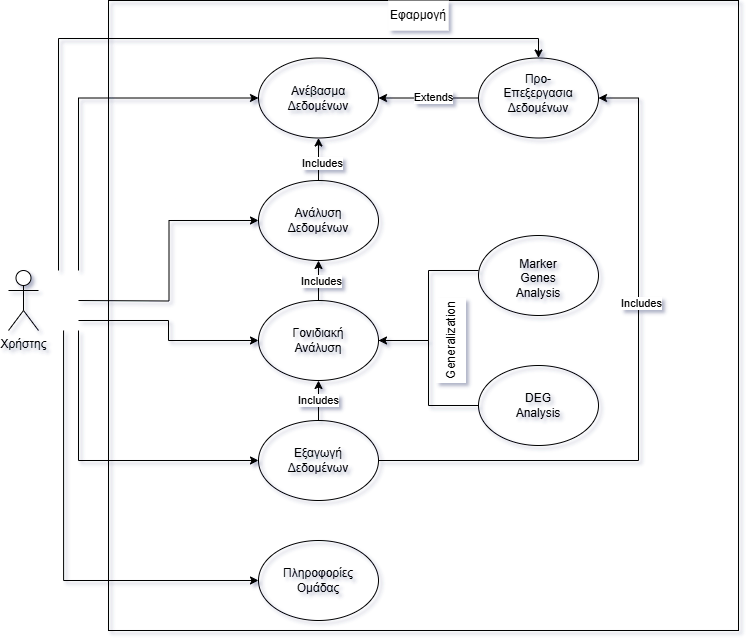
\includegraphics[width=0.9\textwidth]{images/Use_Case_Diagram.png}
    \caption{\foreignlanguage{english}{Use Case Diagram} της εφαρμογής}
\end{figure}

\chapter{Ανάλυση της Υλοποίησης με Τεχνικές Λεπτομέρειες}

Η εφαρμογή έχει υλοποιηθεί σε \foreignlanguage{english}{Python} με χρήση των βιβλιοθηκών \foreignlanguage{english}{Streamlit, Scanpy, anndata, Plotly, Pandas, Matplotlib, NumPy, SciPy, seaborn} και \foreignlanguage{english}{HarmonyPy}. Όλη η ροή της εφαρμογής οργανώνεται στο αρχείο \foreignlanguage{english}{\texttt{main.py}}, το οποίο διαχωρίζει τη λειτουργικότητα σε έξι διαδραστικά \foreignlanguage{english}{tabs}.

\section*{0. Ανέβασμα Αρχείου}
Ο χρήστης μπορεί να φορτώσει ένα αρχείο τύπου \foreignlanguage{english}{\texttt{.h5ad}} μέσω του \foreignlanguage{english}{\texttt{file\_uploader}} του \foreignlanguage{english}{Streamlit}. Εφόσον το αρχείο φορτωθεί επιτυχώς, γίνεται άμεση ανάγνωση με τη συνάρτηση \foreignlanguage{english}{\texttt{scanpy.read\_h5ad()}} και το αντικείμενο \foreignlanguage{english}{AnnData} αποθηκεύεται σε \foreignlanguage{english}{\texttt{st.session\_state}}.

Παράλληλα εμφανίζεται συνοπτική προεπισκόπηση μετρικών (αρ. κυττάρων, αρ. γονιδίων), ενώ ο χρήστης έχει δυνατότητα να περιηγηθεί στις εγγραφές του \foreignlanguage{english}{\texttt{adata.obs}} και \foreignlanguage{english}{\texttt{adata.var}} ανά σελίδες.


\section*{1. Προεπεξεργασία}
Περιλαμβάνει τον καθαρισμό των δεδομένων και τις παρακάτω λειτουργίες:
\begin{itemize}
  \item \foreignlanguage{english}{\texttt{filter\_cells}, \texttt{filter\_genes}} για φιλτράρισμα βάση τιμής που δίνεται από τον χρήστη.
  \item Αφαίρεση γονιδίων \foreignlanguage{english}{\texttt{MT-}}, \foreignlanguage{english}{\texttt{ERCC}} με χρήση προθέματος.
  \item Κανονικοποίηση με \foreignlanguage{english}{\texttt{normalize\_total}} και μετασχηματισμός \foreignlanguage{english}{\texttt{log1p}}.
  \item Επιλογή γονιδίων υψηλής διακύμανσης με \foreignlanguage{english}{\texttt{highly\_variable\_genes}}.
  \item Κανονικοποίηση τιμών μέσω \foreignlanguage{english}{\texttt{scale}}.
\end{itemize}

\section*{2. \foreignlanguage{english}{PCA, Clustering, UMAP, Harmony}}
Ανάλυση κύριων συνιστωσών \foreignlanguage{english}{(clusters)}  και ομαδοποίηση:
\begin{itemize}
  \item Υπολογισμός \foreignlanguage{english}{\texttt{PCA}} με δυνατότητα επιλογής αριθμού συνιστωσών \foreignlanguage{english}{(clusters)}.
  \item Δημιουργία γράφου γειτνίασης και \foreignlanguage{english}{clustering} με τον αλγόριθμο \foreignlanguage{english}{Leiden}.
  \item Χρήση \foreignlanguage{english}{UMAP} για \foreignlanguage{english}{2D ή 3D} προβολή.
  \item Προαιρετικά: διόρθωση \foreignlanguage{english}{batch effect} με \foreignlanguage{english}{\texttt{harmony\_integrate}} από το \foreignlanguage{english}{scanpy.external}.
\end{itemize}

\section*{3. \foreignlanguage{english}{Marker Genes}}
Ανίχνευση γονιδίων που διαφοροποιούν τα \foreignlanguage{english}{clusters}:
\begin{itemize}
  \item Μέθοδοι: \foreignlanguage{english}{\texttt{logreg}}, \foreignlanguage{english}{\texttt{wilcoxon}}, \foreignlanguage{english}{\texttt{t-test}} μέσω \foreignlanguage{english}{\texttt{rank\_genes\_groups}}.
  \item Οπτικοποιήσεις με \foreignlanguage{english}{dotplot}, \foreignlanguage{english}{heatmap} και \foreignlanguage{english}{violin}.
\end{itemize}

\section*{4. \foreignlanguage{english}{DEG (Differential Expression)}}
Ανάλυση μεταξύ δύο ομάδων:
\begin{itemize}
  \item Επιλογή ομάδας ενδιαφέροντος και ομάδας αναφοράς (\foreignlanguage{english}{group vs. reference}).
  \item Χρήση της \foreignlanguage{english}{Wilcoxon} για εξαγωγή διαφορικά εκφραζόμενων γονιδίων.
  \item Δημιουργία \foreignlanguage{english}{Volcano plot} με χρωματική ένδειξη για \foreignlanguage{english}{UP}, \foreignlanguage{english}{DOWN} και \foreignlanguage{english}{NS (not significant)} γονίδια.
\end{itemize}

\section*{5. Εξαγωγή Αποτελεσμάτων}
Ο χρήστης μπορεί να:
\begin{itemize}
  \item Κατεβάσει \foreignlanguage{english}{preprocessed} δεδομένα σε \foreignlanguage{english}{.h5ad}.
  \item Εξαγάγει πίνακες \foreignlanguage{english}{DEGs} σε \foreignlanguage{english}{CSV/XLSX}.
  \item Κατεβάσει εικόνες \foreignlanguage{english}{UMAP}, \foreignlanguage{english}{Volcano}, \foreignlanguage{english}{Heatmap, Dotplot, Violin}.
\end{itemize}

Όλες οι ενέργειες και τα \foreignlanguage{english}{intermediate data} αποθηκεύονται σε \foreignlanguage{english}{\texttt{st.session\_state}}, εξασφαλίζοντας διατήρηση κατάστασης μεταξύ των \foreignlanguage{english}{tabs} και της αλληλεπίδρασης του χρήστη.

\chapter{Οπτικοποιήσεις και Αποτελέσματα}

Η εφαρμογή προσφέρει δυναμικές οπτικοποιήσεις για όλα τα στάδια της ανάλυσης:

\begin{itemize}
  \item \foreignlanguage{english}{UMAP} πριν και μετά την ανάλυση, με χρωματισμούς κατά \foreignlanguage{english}{`batch`} ή \foreignlanguage{english}{`celltype`}.
  \item \foreignlanguage{english}{3D} προβολές των \foreignlanguage{english}{clusters} με δυνατότητα περιστροφής.
  \item Αποτελέσματα προεπεξεργασίας σε μορφή ενημερωτικών καρτών.
  \item \foreignlanguage{english}{Volcano plot} με \foreignlanguage{english}{logFC} και \foreignlanguage{english}{p-value} για \foreignlanguage{english}{DEG}.
  \item \foreignlanguage{english}{Dotplot/Violin/Heatmap} για \foreignlanguage{english}{marker genes}.
\end{itemize}

Όλες οι εικόνες είναι εξαγώγιμες ως \foreignlanguage{english}{PNG} από την ίδια την εφαρμογή.

\section*{Ενδεικτικές Οπτικοποιήσεις}

\begin{figure}[!htb]
  \centering
  \begin{minipage}[t]{0.46\textwidth}
    \centering
    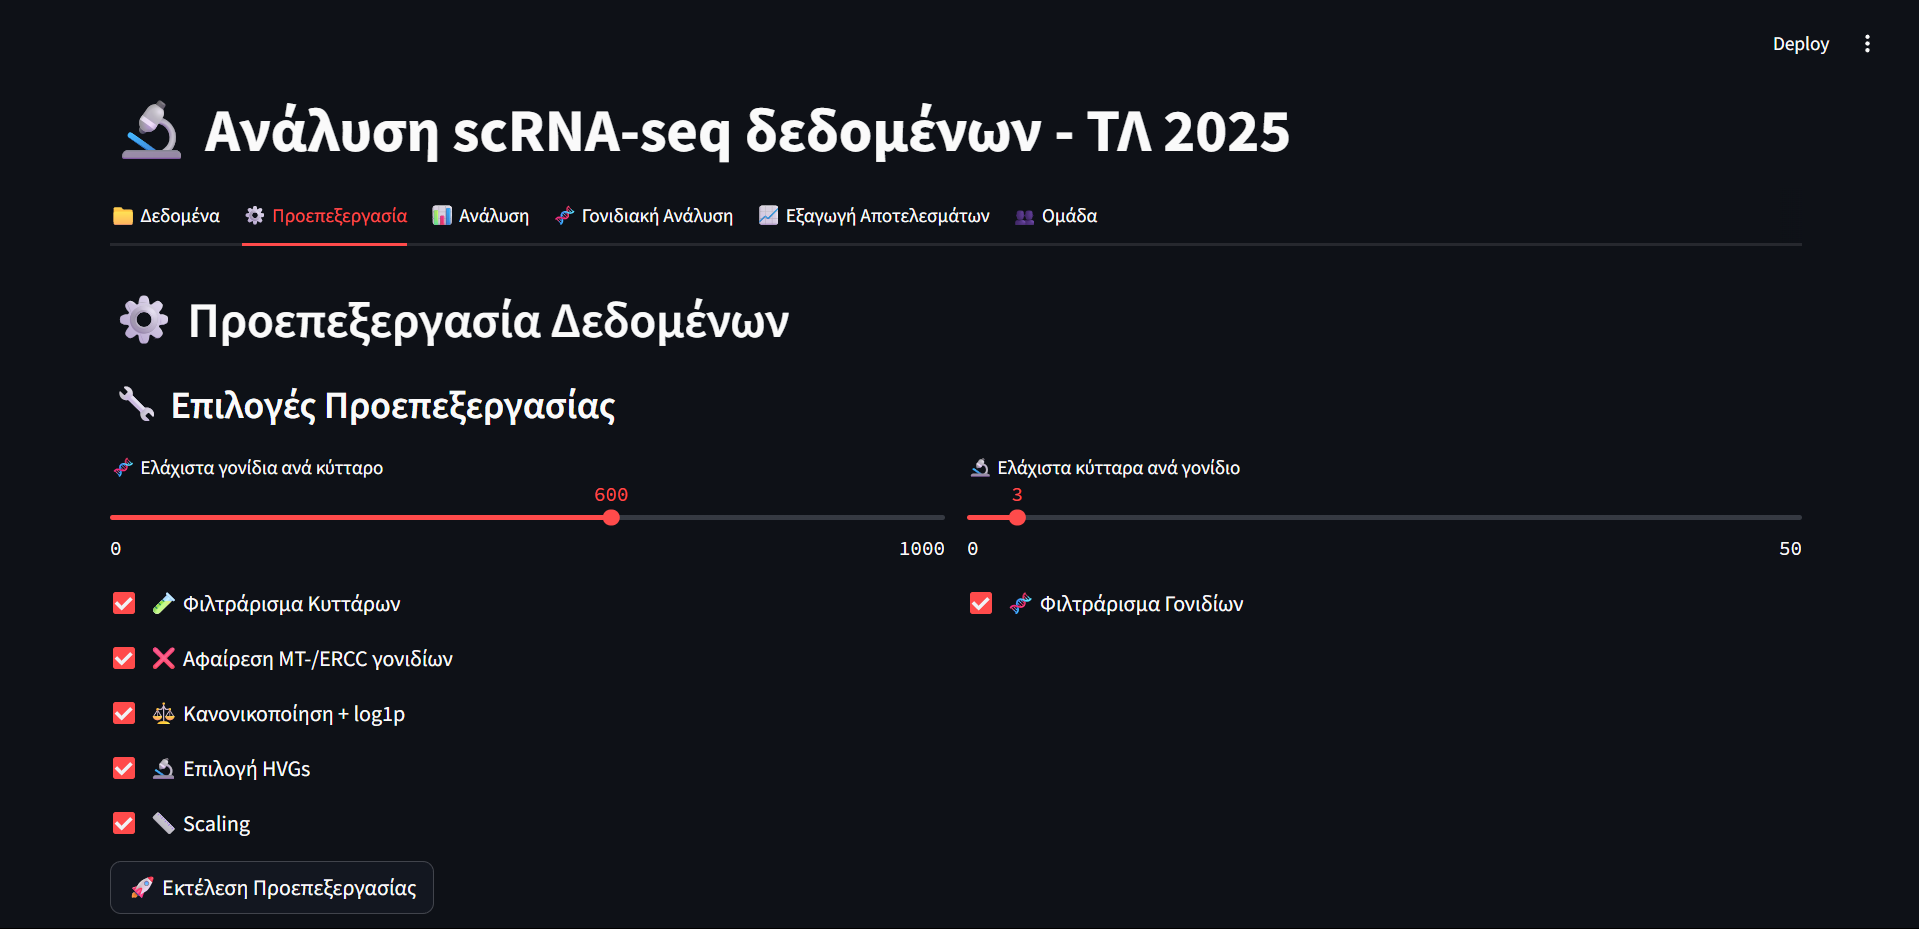
\includegraphics[width=\textwidth]{images/Preprocessing.png}
    \caption*{\small Οθόνη Επιλογών Προεπεξεργασίας}
  \end{minipage}
  \hfill
  \begin{minipage}[t]{0.46\textwidth}
    \centering
    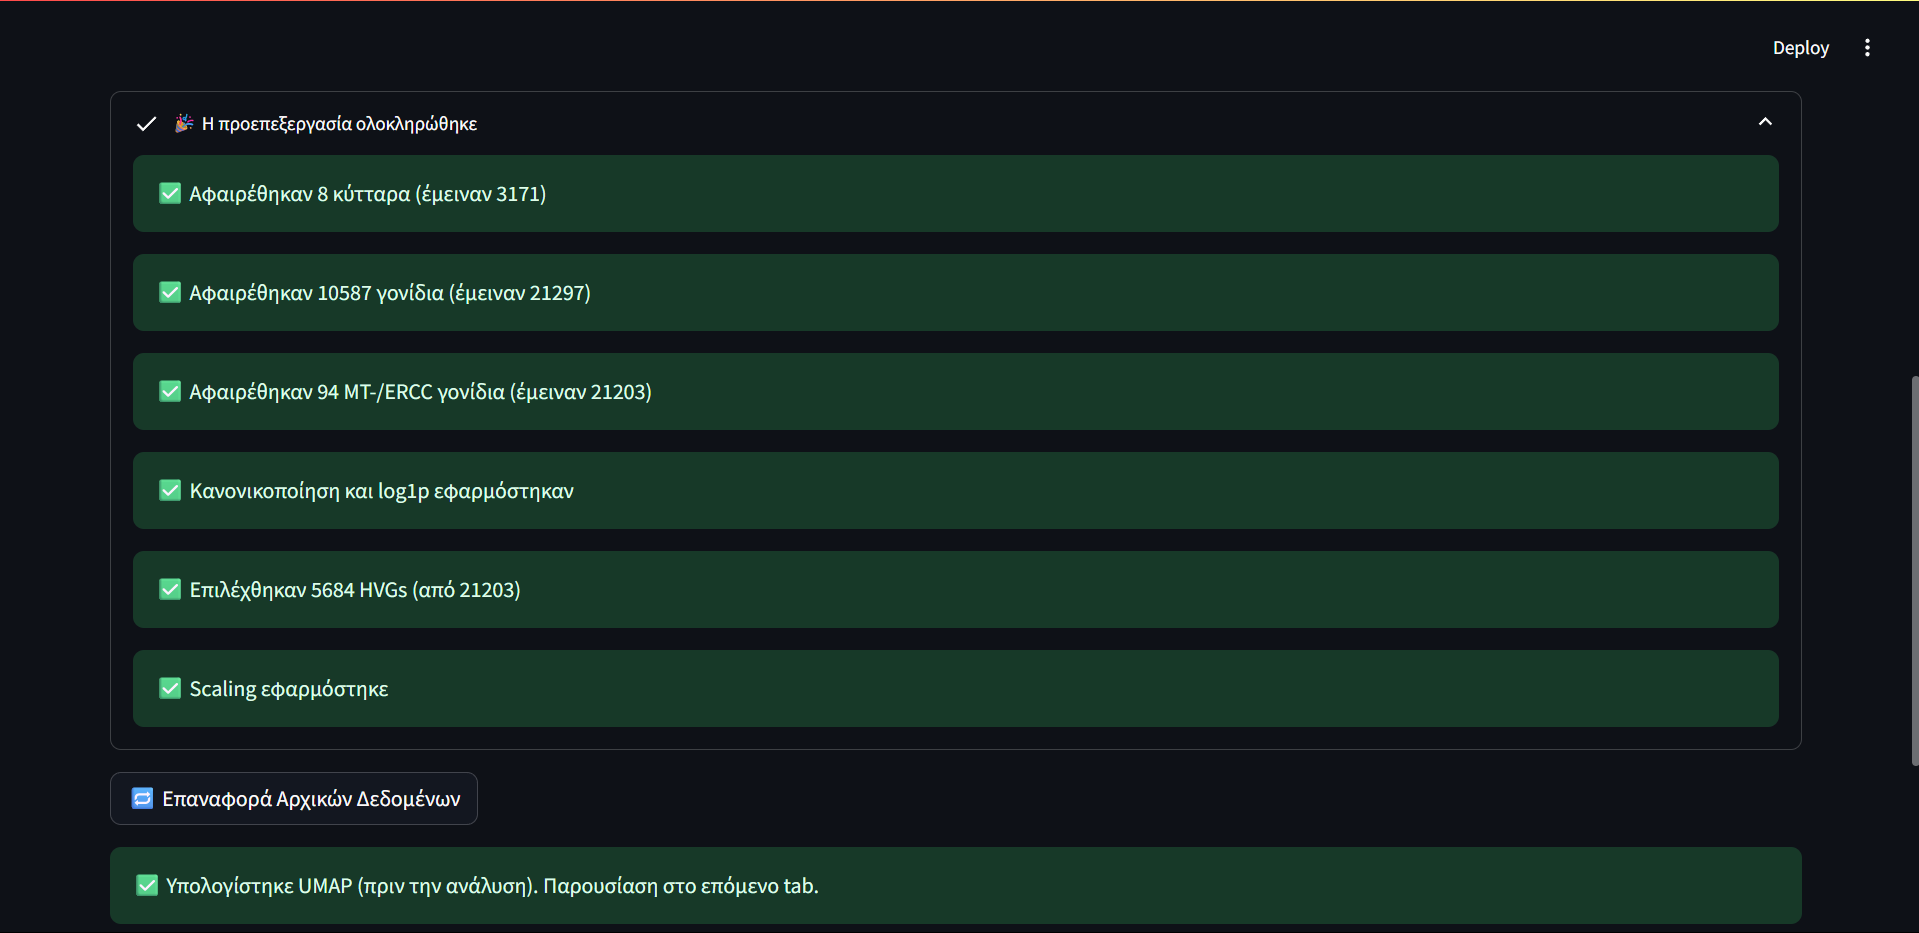
\includegraphics[width=\textwidth]{images/Preprocessing_Result.png}
    \caption*{\small Αποτελέσματα Προεπεξεργασίας}
  \end{minipage}
\end{figure}

\begin{figure}[!htb]
  \centering
  \begin{minipage}[t]{0.46\textwidth}
    \centering
    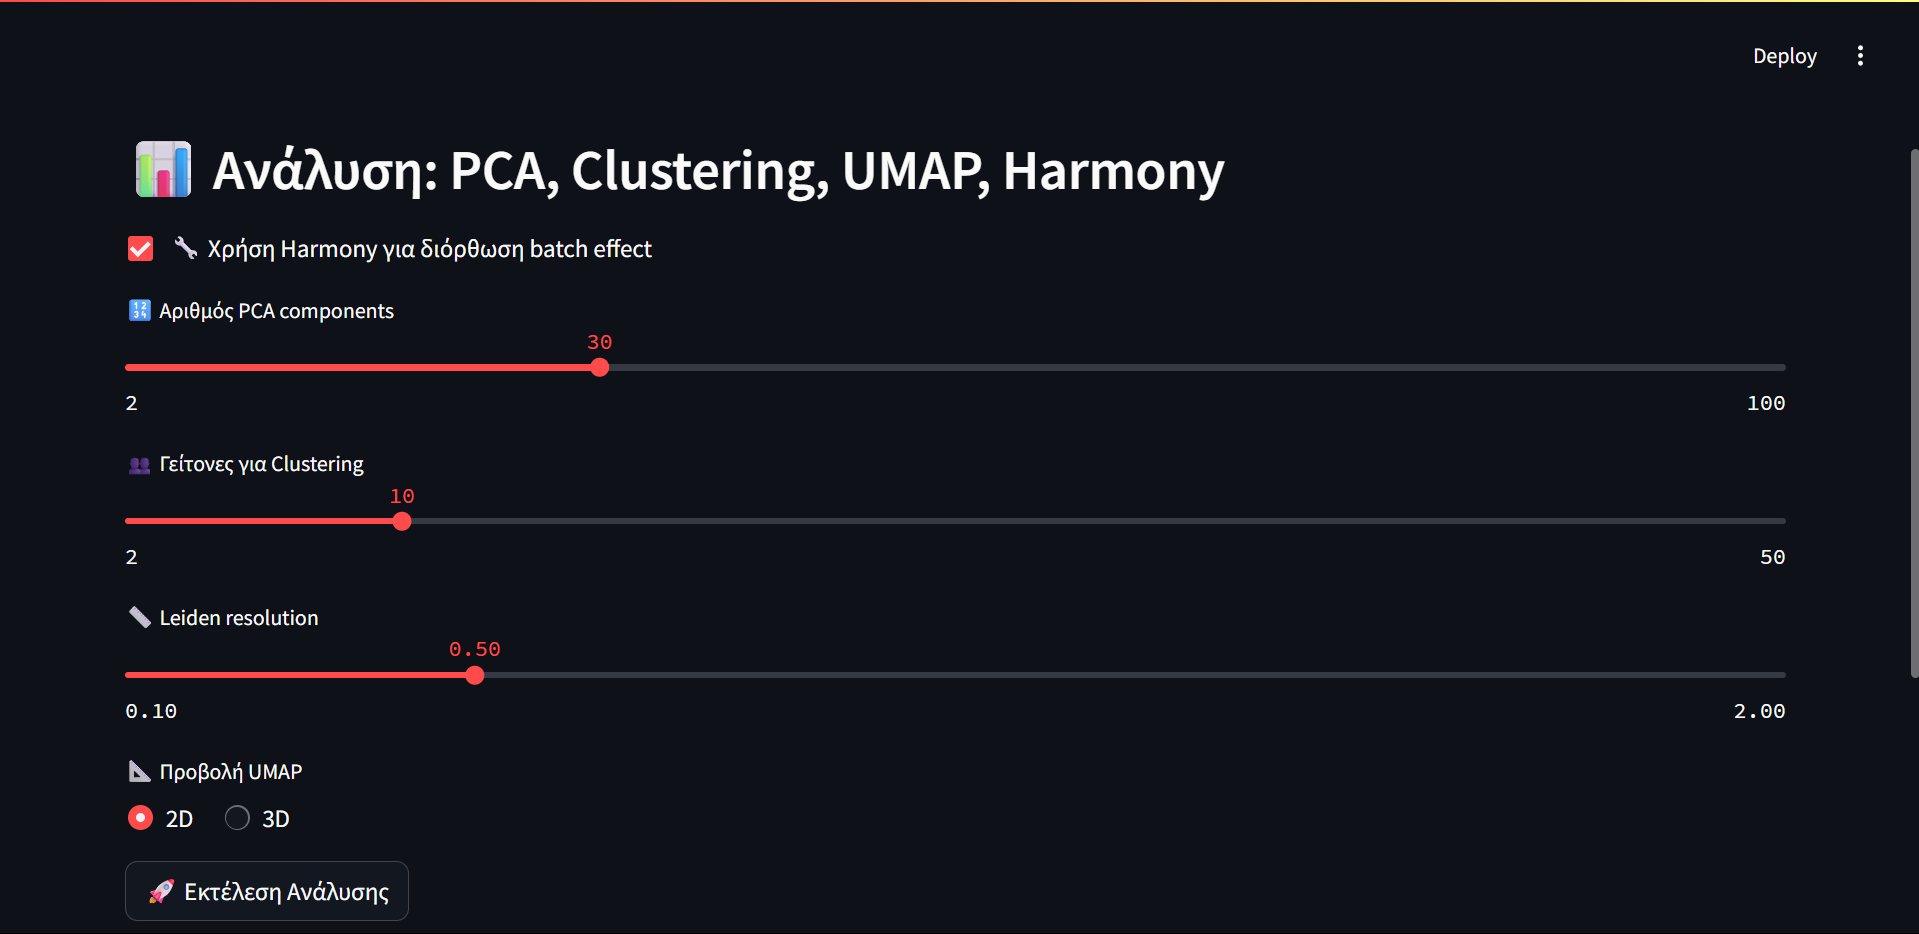
\includegraphics[width=\textwidth]{images/Analysis.png}
    \caption*{\small Παράμετροι Ανάλυσης}
  \end{minipage}
  \hfill
  \begin{minipage}[t]{0.46\textwidth}
    \centering
    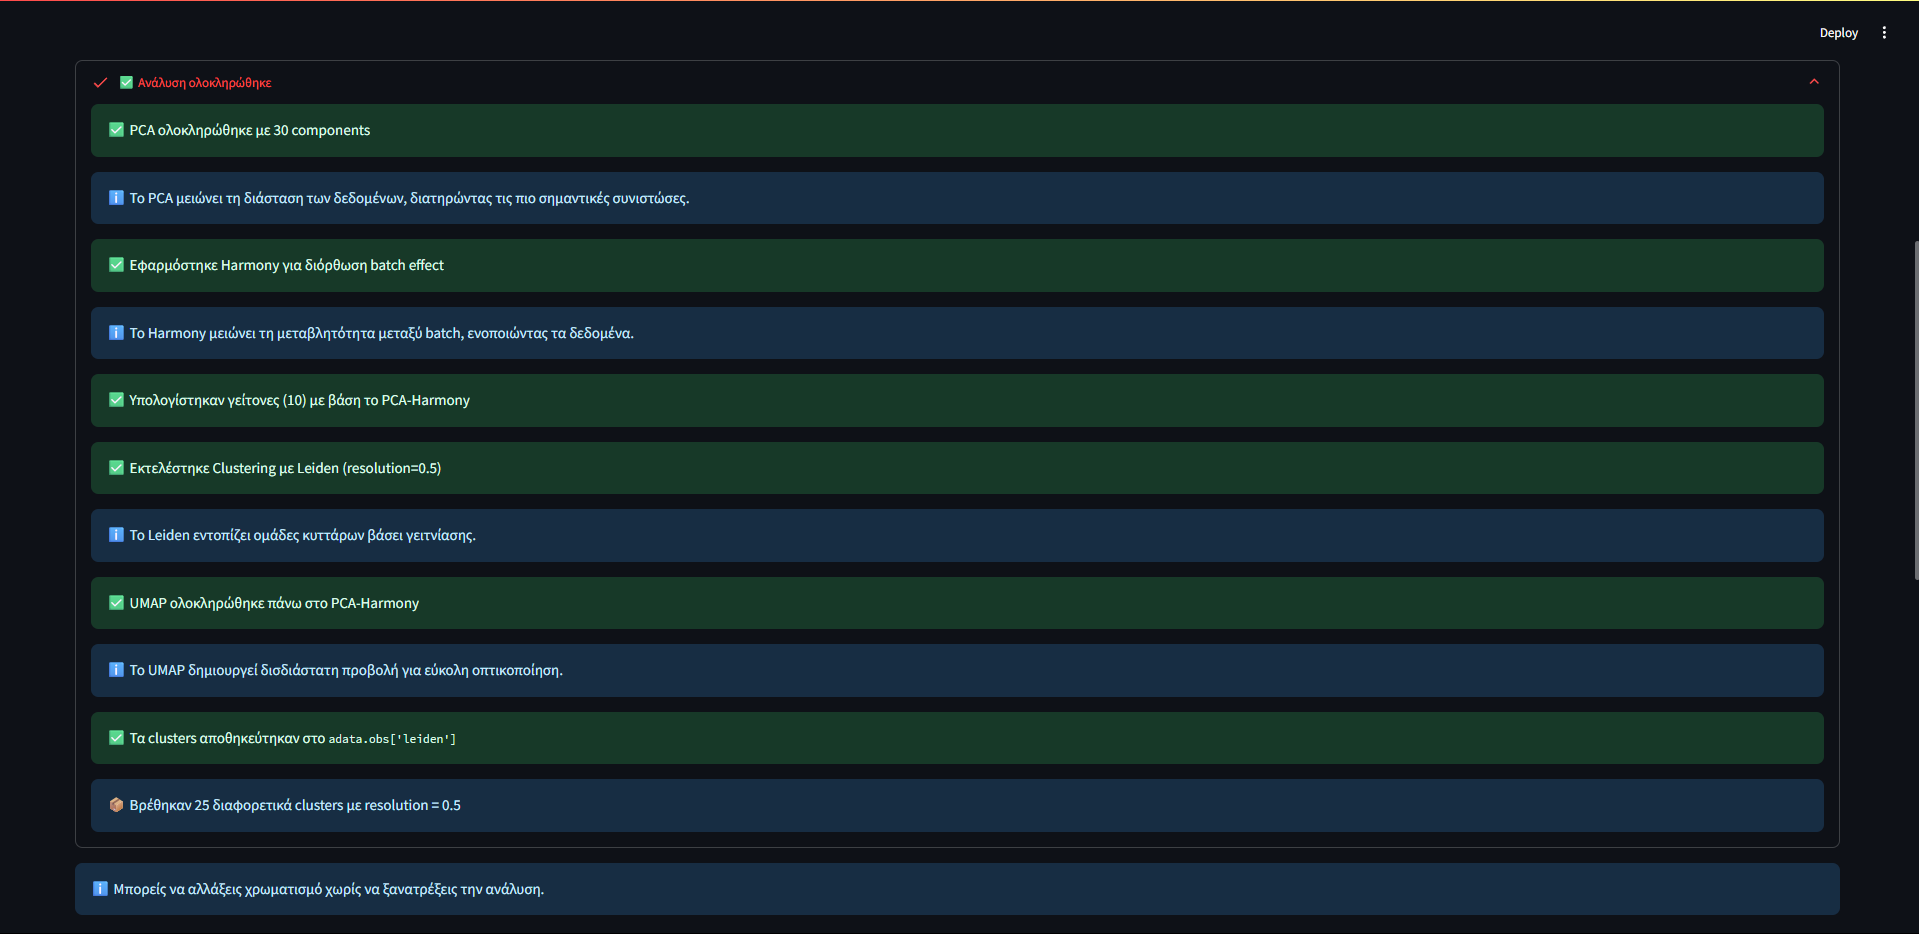
\includegraphics[width=\textwidth]{images/Analysis_Results1.png}
    \caption*{\small Αποτελέσματα \foreignlanguage{english}{PCA \& Harmony}}
  \end{minipage}
\end{figure}

\begin{figure}[!htb]
  \centering
  \begin{minipage}[t]{0.46\textwidth}
    \centering
    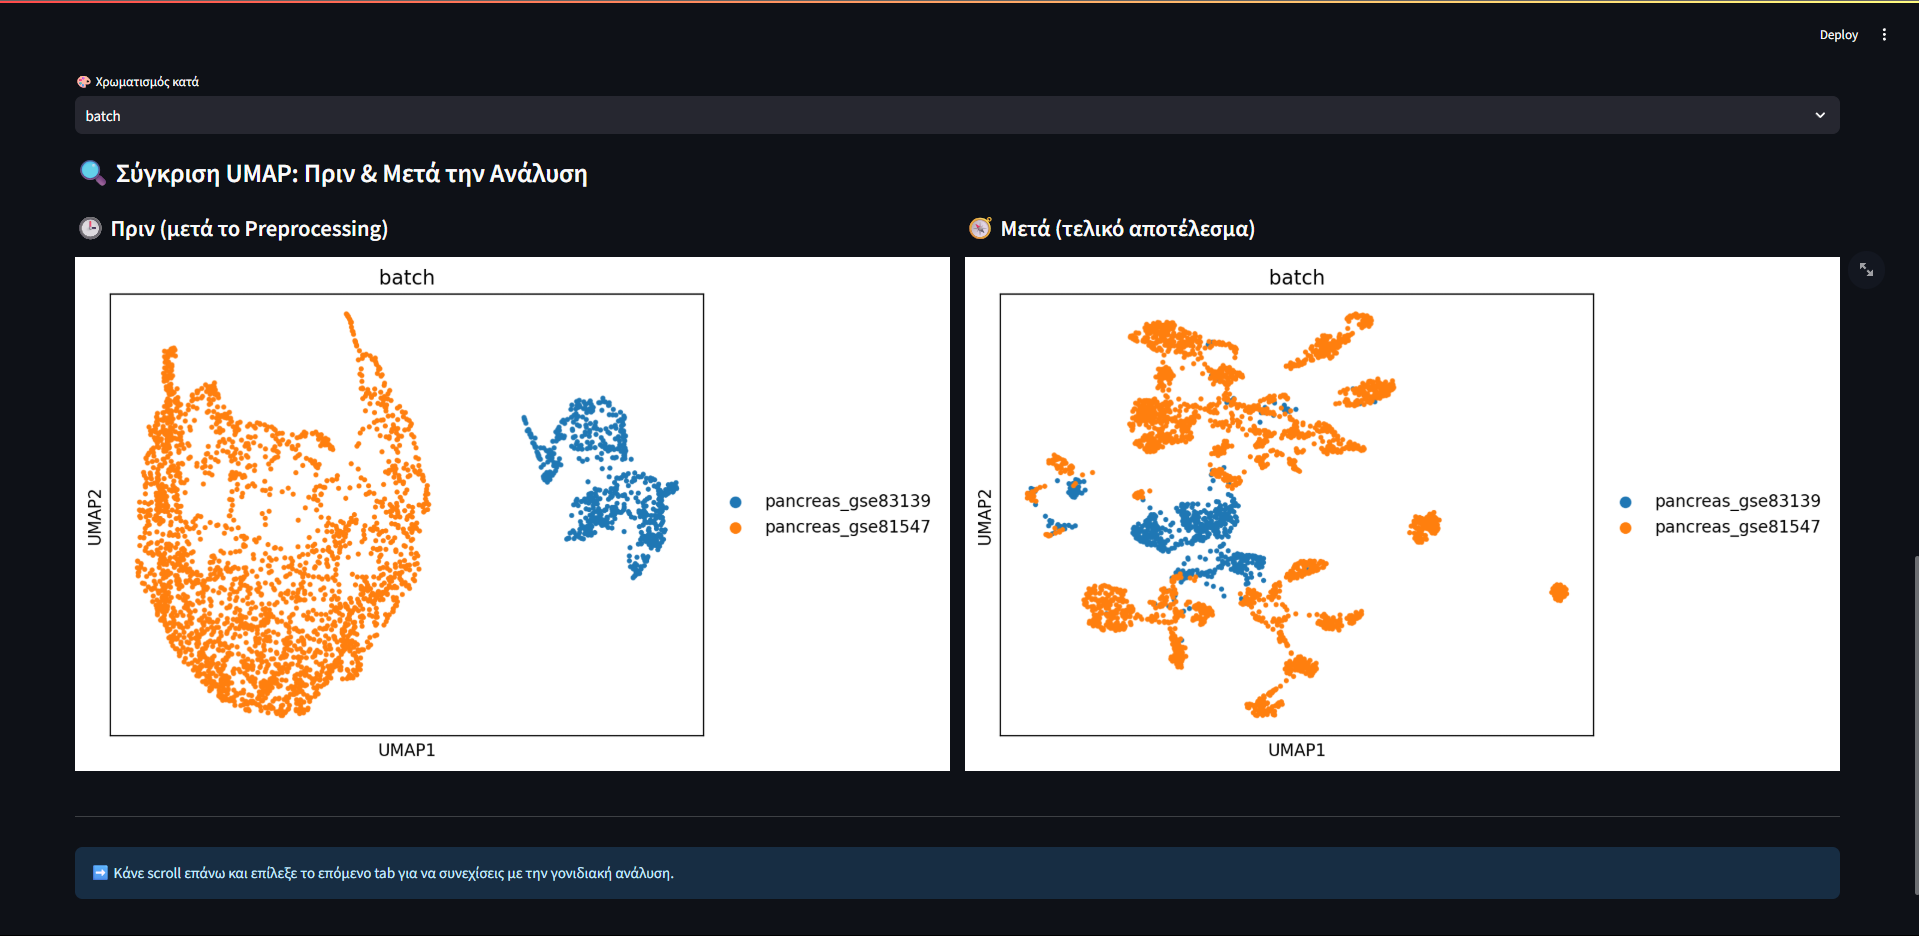
\includegraphics[width=\textwidth]{images/Analysis_Results2.png}
    \caption*{\small \foreignlanguage{english}{UMAP 2D} πριν \& μετά - \foreignlanguage{english}{Batch}}
  \end{minipage}
  \hfill
  \begin{minipage}[t]{0.46\textwidth}
    \centering
    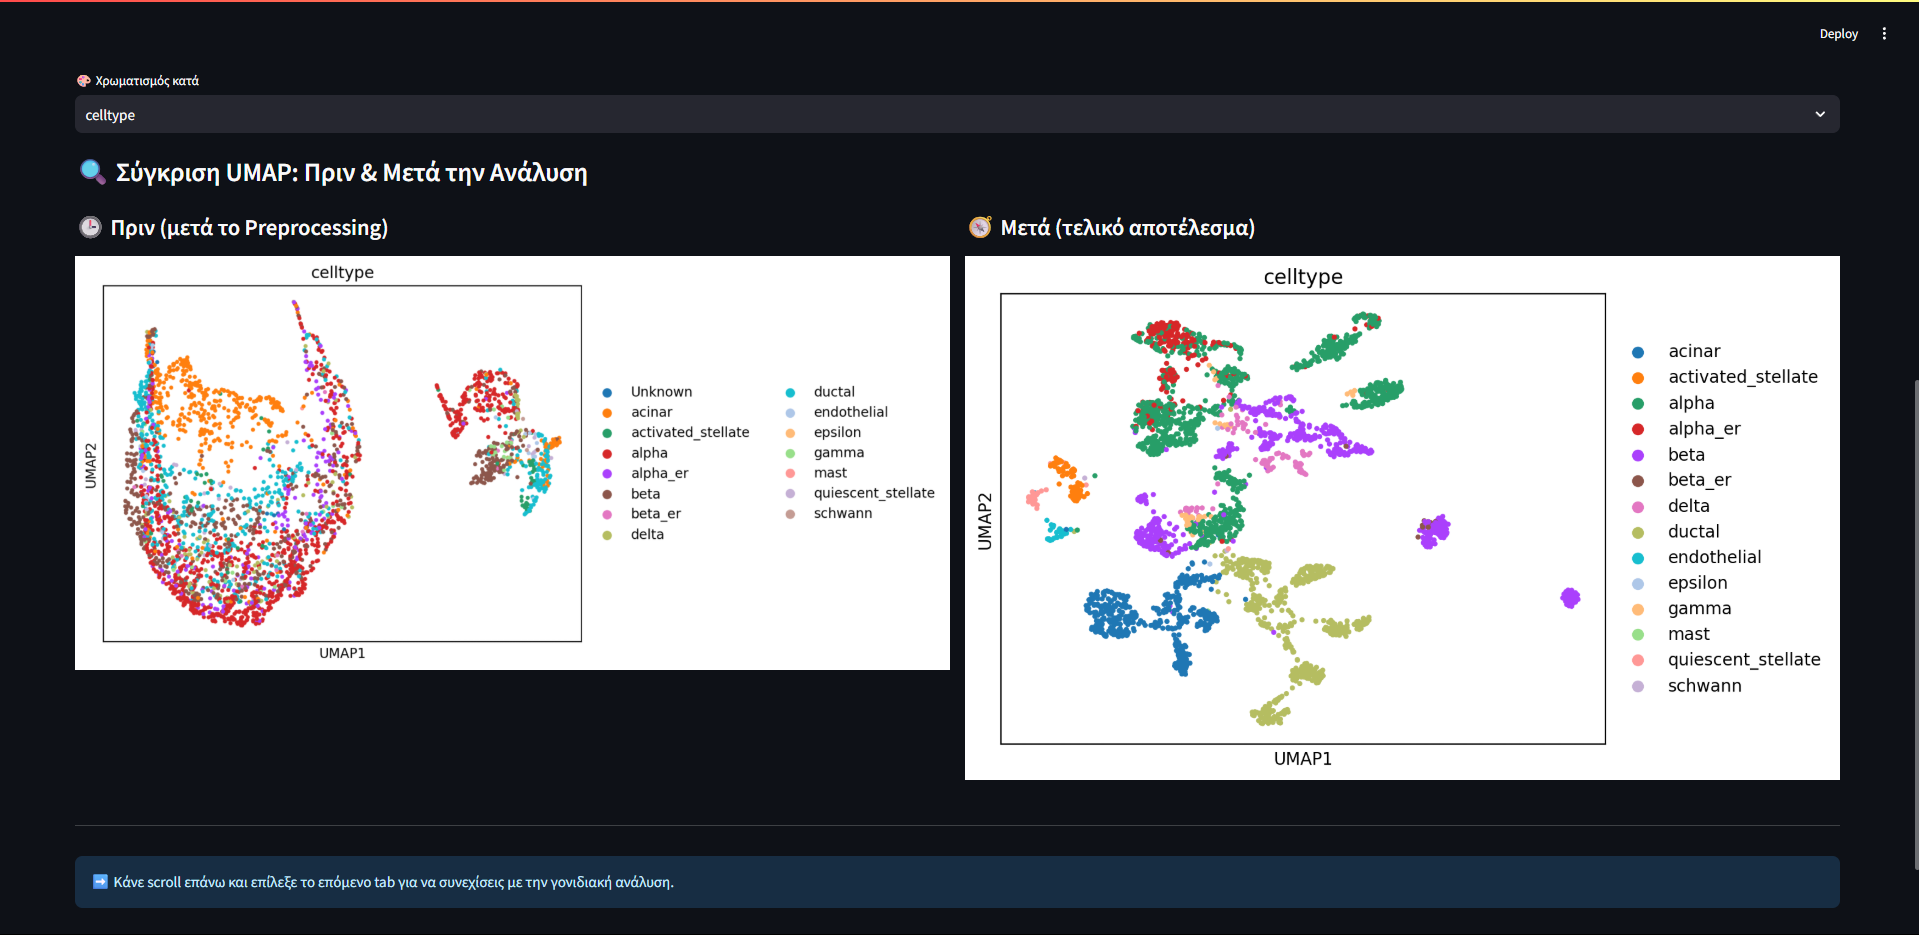
\includegraphics[width=\textwidth]{images/Analysis_Results3.png}
    \caption*{\small \foreignlanguage{english}{UMAP 2D} πριν \& μετά - \foreignlanguage{english}{Celltype}}
  \end{minipage}
\end{figure}

\begin{figure}[!htb]
  \centering
  \begin{minipage}[t]{0.46\textwidth}
    \centering
    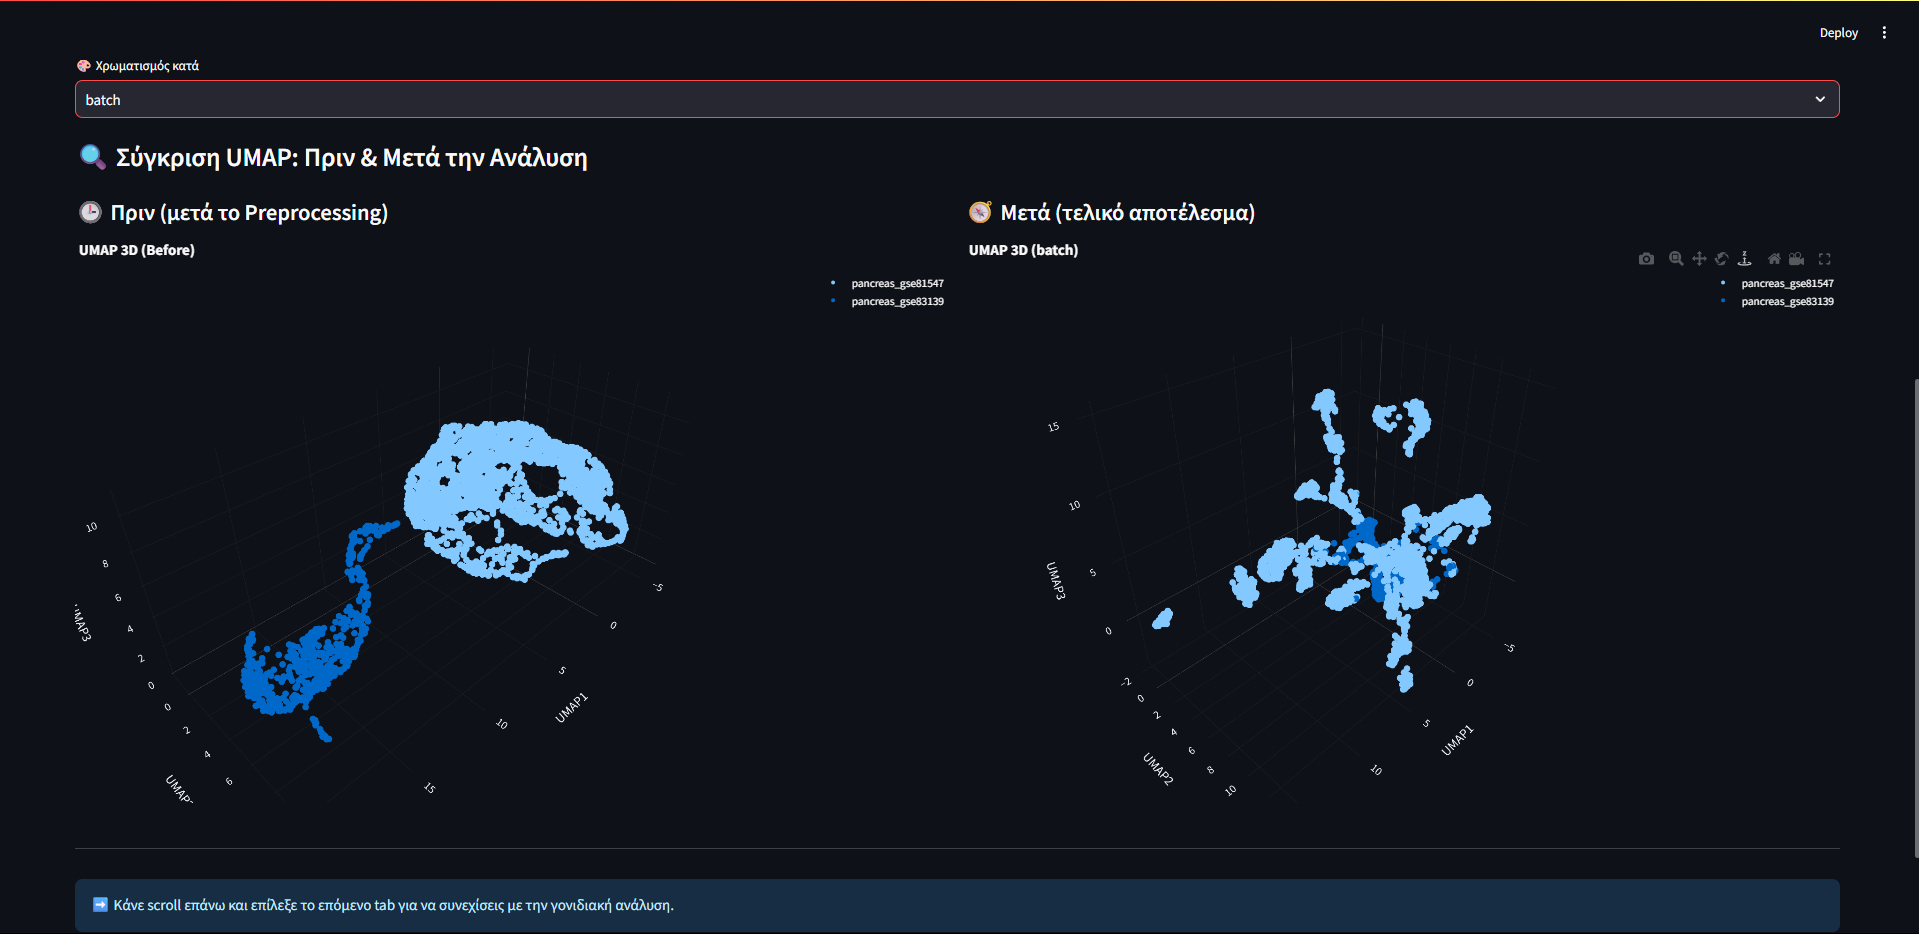
\includegraphics[width=\textwidth]{images/Analysis_Results4.png}
    \caption*{\small \foreignlanguage{english}{UMAP 3D} πριν \& μετά - \foreignlanguage{english}{Batch}}
  \end{minipage}
  \hfill
  \begin{minipage}[t]{0.46\textwidth}
    \centering
    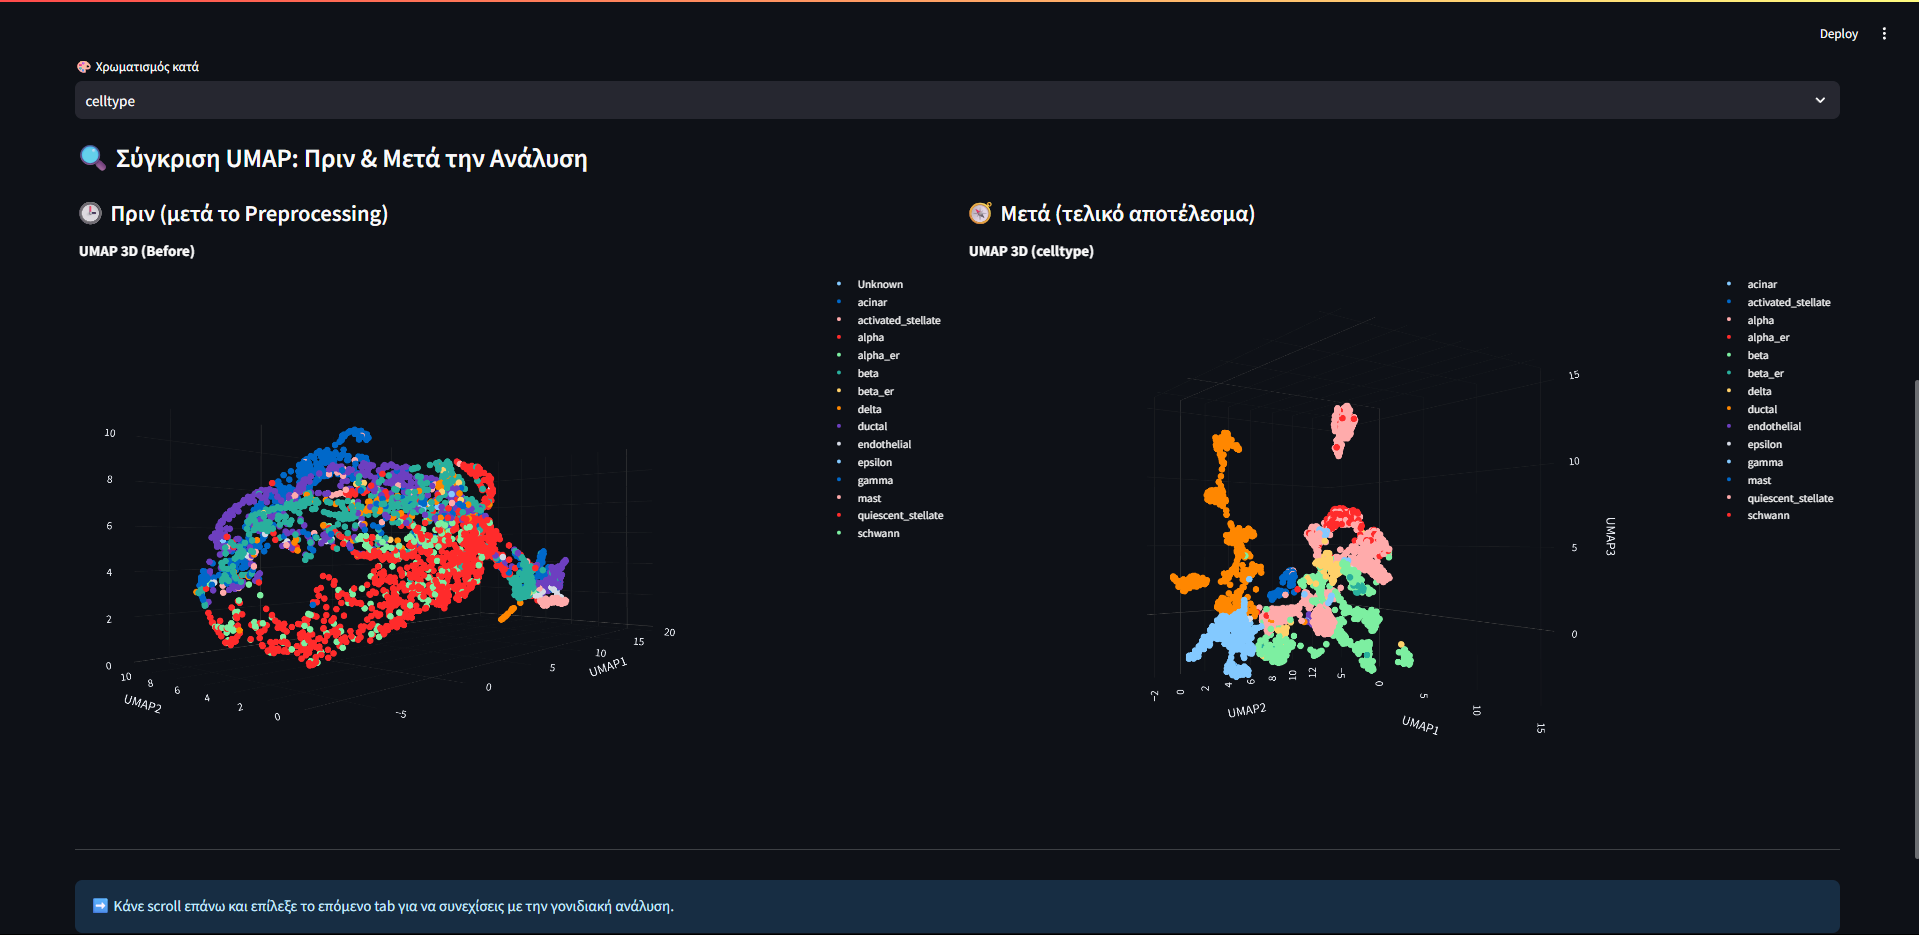
\includegraphics[width=\textwidth]{images/Analysis_Results5.png}
    \caption*{\small \foreignlanguage{english}{UMAP 3D} πριν \& μετά - \foreignlanguage{english}{Celltype}}
  \end{minipage}
\end{figure}

\begin{figure}[!htb]
  \centering
  \begin{minipage}[t]{0.46\textwidth}
    \centering
    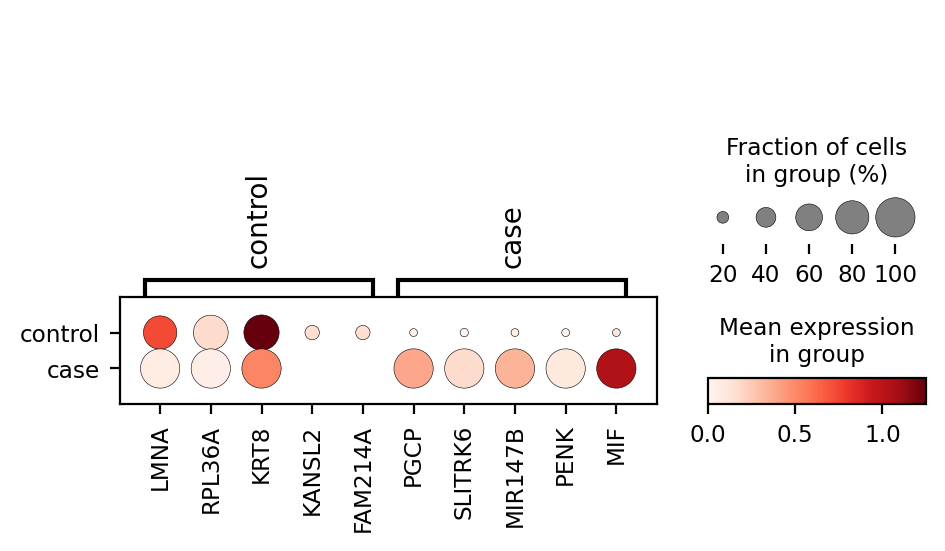
\includegraphics[width=\textwidth]{images/Marker_Gens_Dotplot.png}
    \caption*{\small \foreignlanguage{english}{Dotplot Marker Genes}}
  \end{minipage}
  \hfill
  \begin{minipage}[t]{0.46\textwidth}
    \centering
    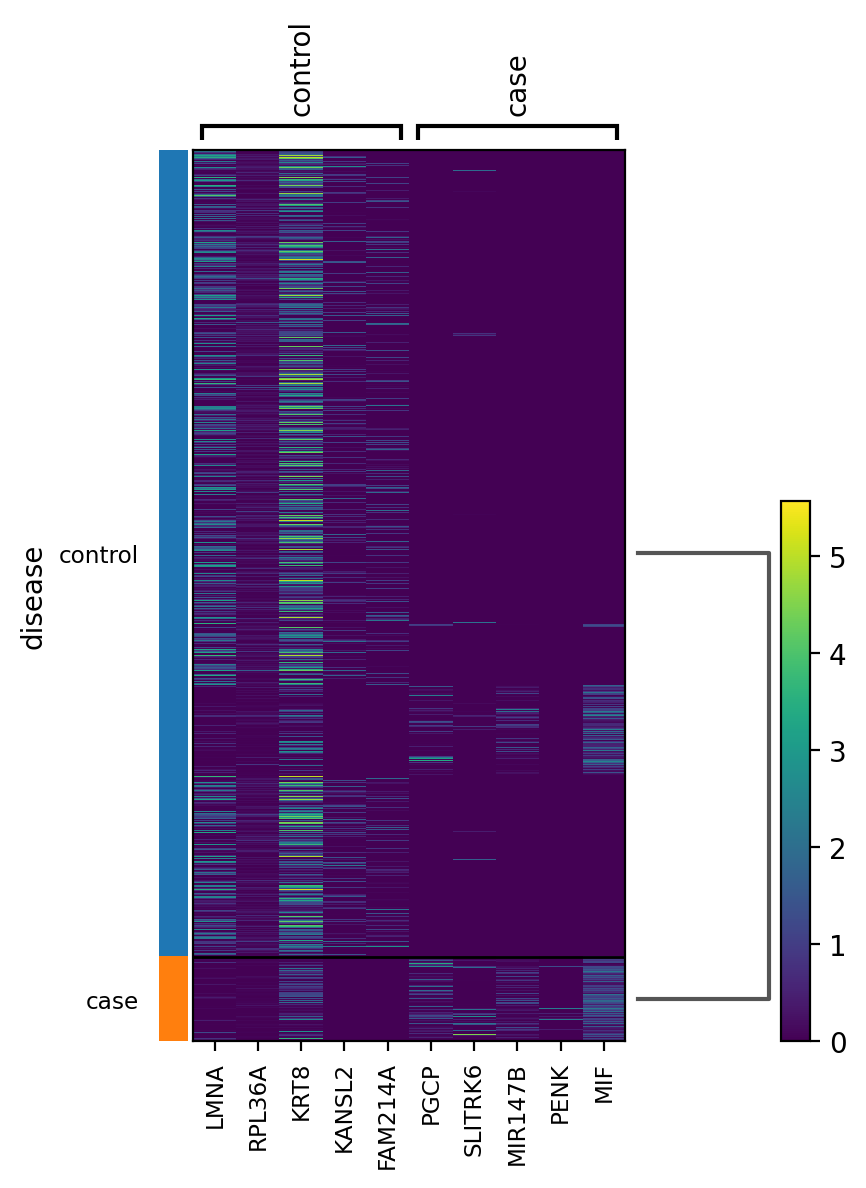
\includegraphics[width=\textwidth]{images/Marker_Genes_Heatmap.png}
    \caption*{\small \foreignlanguage{english}{Heatmap Marker Genes}}
  \end{minipage}
\end{figure}

\begin{figure}[!htb]
  \centering
  \begin{minipage}[t]{0.46\textwidth}
    \centering
    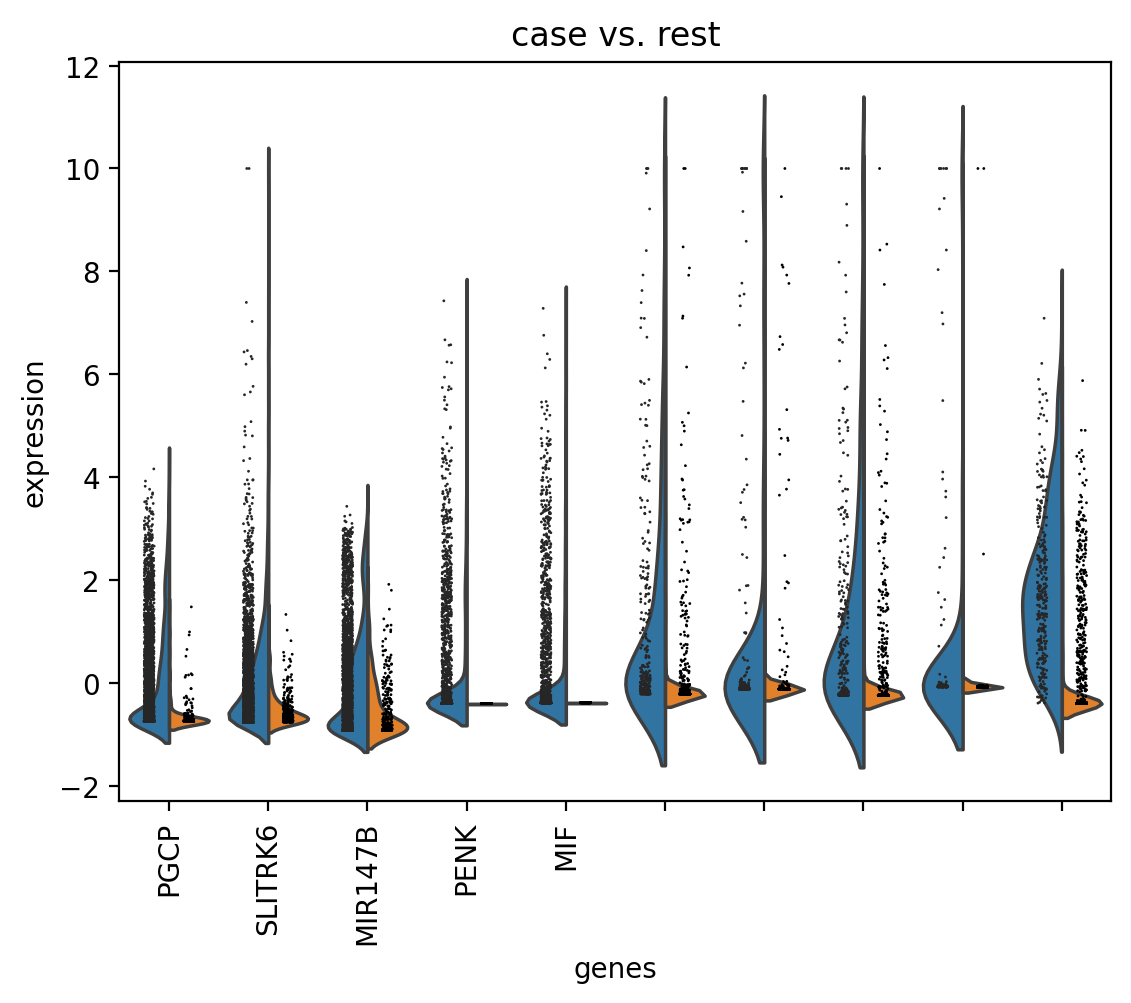
\includegraphics[width=\textwidth]{images/Marker_Genes_Violin.png}
    \caption*{\small \foreignlanguage{english}{Violin Plot Marker Genes}}
  \end{minipage}
  \hfill
  \begin{minipage}[t]{0.60\textwidth}
    \centering
    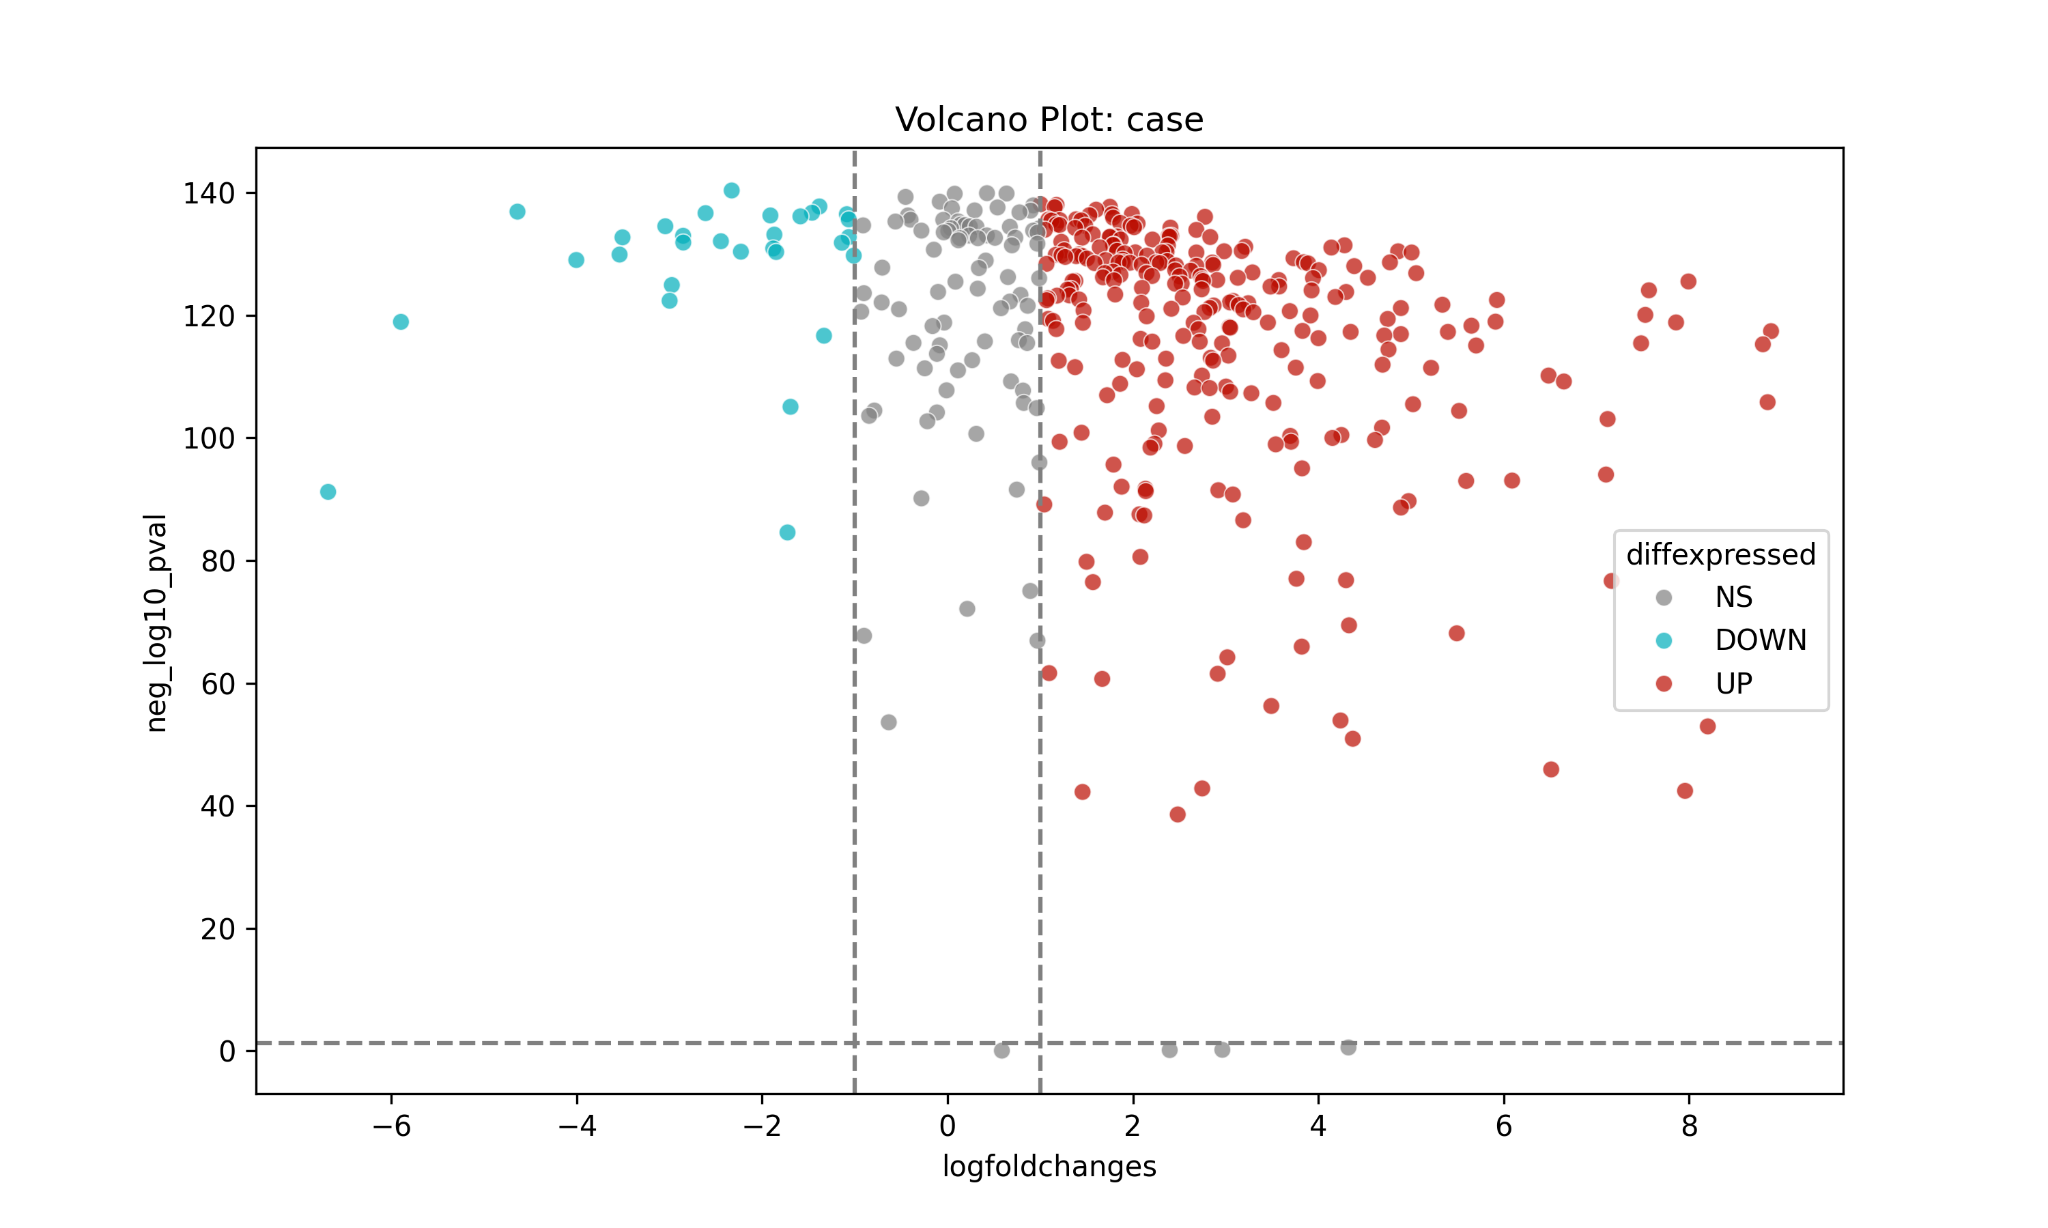
\includegraphics[width=\textwidth]{images/Volcano_Plot.png}
    \caption*{\small \foreignlanguage{english}{Volcano Plot}}
  \end{minipage}
\end{figure}
\chapter{\foreignlanguage{english}{Dockerization} της Εφαρμογής}

Η εφαρμογή έχει υλοποιηθεί ώστε να τρέχει πλήρως απομονωμένα μέσω \foreignlanguage{english}{Docker}, διευκολύνοντας την εγκατάσταση και εκτέλεση σε οποιοδήποτε περιβάλλον.

\section*{Αρχείο \foreignlanguage{english}{Dockerfile}}

Το \foreignlanguage{english}{Dockerfile} βασίζεται στην επίσημη εικόνα \foreignlanguage{english}{\texttt{python:3.11-slim}} και περιλαμβάνει:

\begin{itemize}
  \item Εγκατάσταση εξαρτήσεων από το αρχείο \foreignlanguage{english}{\texttt{requirements.txt}}
  \item Αντιγραφή όλων των απαραίτητων αρχείων στον \foreignlanguage{english}{container}
  \item Ορισμός \foreignlanguage{english}{entrypoint} με την εντολή: \foreignlanguage{english}{\texttt{CMD ["streamlit", "run", "main.py"]}}
\end{itemize}

\section*{Αρχείο \foreignlanguage{english}{requirements.txt}}

Το αρχείο \foreignlanguage{english}{\texttt{requirements.txt}} περιλαμβάνει όλες τις βιβλιοθήκες που απαιτούνται για την εκτέλεση της εφαρμογής. Ενδεικτικά:

\begin{itemize}
  \item \foreignlanguage{english}{streamlit, scanpy, anndata, matplotlib, numpy, pandas}
  \item \foreignlanguage{english}{scipy, plotly, seaborn, harmonypy}
  \item \foreignlanguage{english}{python-igraph, leidenalg, openpyxl, xlsxwriter}
\end{itemize}

\newpage

\section*{Εντολές Εκτέλεσης}

Η δημιουργία και εκτέλεση του \foreignlanguage{english}{Docker container} γίνεται με:

\begin{center}
\begin{alltt}
\selectlanguage{english}
docker build -t scrna-app .

docker run -p 8501:8501 scrna-app
\selectlanguage{greek}
\end{alltt}
\end{center}

Αυτό καθιστά την εφαρμογή διαθέσιμη στη διεύθυνση: \foreignlanguage{english}{\texttt{http://localhost:8501}}

\section*{Αρχείο \foreignlanguage{english}{.dockerignore}}

Το αρχείο \foreignlanguage{english}{\texttt{.dockerignore}} περιλαμβάνει τα εξής:

\begin{itemize}
  \item \foreignlanguage{english}{\texttt{.git/}} – αποφυγή μεταφοράς \foreignlanguage{english}{git} ιστορικού
  \item \foreignlanguage{english}{\texttt{.vscode/}} – ρυθμίσεις \foreignlanguage{english}{editor}
  \item \foreignlanguage{english}{\texttt{\_\_pycache\_\_/}} – προερμηνευμένα αρχεία \foreignlanguage{english}{Python}
\end{itemize}

Με αυτόν τον τρόπο μειώνεται το μέγεθος του \foreignlanguage{english}{Docker image} και διασφαλίζεται καθαρό περιβάλλον εκτέλεσης.

\chapter{Αποθετήριο στο \foreignlanguage{english}{GitHub}}

Ο πηγαίος κώδικας της εφαρμογής είναι διαθέσιμος στο \foreignlanguage{english}{GitHub}, στο εξής αποθετήριο:

\begin{itemize}
  \item \foreignlanguage{english}{\textbf{Link:} \url{https://github.com/chriskarydis/scRNA_seq_Pipeline}}
  \item Περιέχει: \foreignlanguage{english}{`main.py`, `Dockerfile`, `requirements.txt`, `.dockerignore`, `README.md`}
  \item Το \foreignlanguage{english}{`README.md`} περιλαμβάνει οδηγίες εγκατάστασης, τρέξιμο μέσω \foreignlanguage{english}{Docker}, και παραδείγματα αρχείων.
\end{itemize}

Ο χρήστης μπορεί να κλωνοποιήσει το \foreignlanguage{english}{repository} και να εκτελέσει την εφαρμογή είτε τοπικά είτε μέσω \foreignlanguage{english}{Docker} σε περιβάλλον παραγωγής.

\appendix
% \include{appendix/appendixA}

\printbibliography[heading=bibintoc]

\end{document}
